%% template for IEICE Transactions
%% v2.1 [2015/10/31]
\documentclass[paper]{ieice}
%\documentclass[invited]{ieice}
%\documentclass[position]{ieice}
%\documentclass[survey]{ieice}
%\documentclass[invitedsurvey]{ieice}
%\documentclass[review]{ieice}
%\documentclass[tutorial]{ieice}
%\documentclass[letter]{ieice}
%\documentclass[brief]{ieice}
%\usepackage[dvips]{graphicx}
%\usepackage[pdftex]{graphicx,xcolor}
\usepackage[dvipdfmx]{graphicx,xcolor}
\usepackage[fleqn]{amsmath}
\usepackage{newtxtext}
\usepackage[varg]{newtxmath}

\setcounter{page}{1}
%\breakauthorline{}% breaks lines after the n-th author

\field{}
%\SpecialIssue{}
%\SpecialSection{}
%\theme{}
\title{}
%\title[title for header]{title}
%\titlenote{}
\authorlist{%
 \authorentry{Shun Okuhara}{}{}\MembershipNumber{}
 \authorentry{Takayuki Ito}{membership}{affiliate label}\MembershipNumber{}
% \authorentry{name}{membership}{affiliate label}[present affiliate label]\MembershipNumber{}
% \authorentry[e-mail address]{name}{membership}{affiliate label}\MembershipNumber{}
% \authorentry[e-mail address]{name}{membership}{affiliate label}[present affiliate label]\MembershipNumber{}
}
\affiliate[affiliate label]{The author is with the 
}
%\paffiliate[present affiliate label]{Presently, the author is with the }

\received{2015}{1}{1}
\revised{2015}{1}{1}

%% <local definitions here>

%% </local definitions here>

\begin{document}
\maketitle
\begin{summary}
This paper presents an explainable concession process based on constraint relaxation in multi-agent negotiation. Automated negotiation has been studied widely and is the promising technology for the future smart city where multiple heterogeneous agents, like driver-less cars, are conflicting and collaborating.
There are a lot of studies on negotiating agents including international competitions.
The problem is that most of the proposed negotiating agents employ ad-hoc conceding process, where basically they are adjusting threshold to accept their opponents offers. Because it is just adjusting a threshold, it is very difficult to show how and what the agent conceded even after agreement. In this paper, we propose an explainable concession process by using a constraint relaxation process. Here, an agent changes its belief not to believe some constraint so that he/she can accept its opponent offer. Our experimental results demonstrate that our method can work 
\end{summary}
\begin{keywords}
Automated negotiating agents,
compromise,
agreement
\end{keywords}

\section{Introduction}
%
Automated negotiating agents has been studied very widerly in the area of multiagent systems\cite{bai2017multi}, \cite{fukuta2016recent}, \cite{fujita2015next}, \cite{marsa2014novel}, \cite{ito2013complex}, \cite{ito2011new}, \cite{ito2010innovations}, \cite{ito2009advances}, \cite{ito2008rational}. Heterogeneous, intelligent and autonomous systems (agents) has been realized in the real society, like self-driving cars. In such a society, multiple agents could have conflicts. Thus it is required to have a social mechanism that make such agents make an agreement to resolve such conflicts through automated negotiation. Many researchers are working on automated negotiating agents in the field of multiagent systems. In particular, international workshops and international competitions are held around 2010. The multi-agent system is one of the most  important technologies of the next generation. Automated negotiation competition ANAC (Automated Negotiating Agents Competition) has been held from 2010 as a testbed for automatic negotiation agent researches. ANAC adopts the multi-issue utility model and the alternating-offer protocol. A lot of negotiating agents are proposed because ANAC changes and extends the rules of negotiations every year. But there are several drawbacks and problems that ANAC competition could not focus on. One of such problems is the explainability of the compromise process. In negotiations,  agents cannot reach an agreement if it is considering only their own profits and interests. Therefore, the compromise strategy is essential to rearch an agreement. Most of the existing automated negotiatiing agents adopted {\it ad-hoc} compromising processes that only adjusting their thresholds to accept the opponent’s offer. Therefore, there was a problem that it was difficult to explain how the compromise was done in the negotaition. It is important if automated negotiating agents are acting with real human in real society because they do need to explain how and why they compromised. For example, if your self-driving car stopped suddenly in the middle of congestion, you want to know its reason. In this paper, in order to solve this problem, we propose a compromise process based on constraint relaxation. A constraint is a basic unit of utility. In other words, in this research, we define the utility space of the agent as a set of constraints that satisfy the issue values and its argument. When a constraint is satisfied, the agent gets an utility value for this constraint. For example, there are issues like the color, price, type when buying a car. These issues are linked by some constraints. Thus, there could be a constraint that says if ``type`` is ``sports car``, then ``color`` should be ``red``. Also, if ``type`` is ``sedan``, then ``color`` is ``white``. Constraints generate value if it is satisfied, but do not generate any value if they are not satisfied. Also, in this paper, we assume {\it shared} issues and {\it individual} issues. In other words, we can say that agents agreed if they have the same issue-value for shared issues. For individual issues, each agent can choose issue-values to make their utility as high as possible. An agent faces a tradeoff between maximizing its own utilty by satisfying the constraint as much as possible while keeping the share value to be the same value as the opponent agent. In order to solve this tradeoff, agents perform to compromise. In this paper, in the compromise process, the agent removes constraints one by one from the set of its own constraints. Then, it try to change their most preferable issue-value of the shared issue. If the agent can change the issue-value to one which is same as the opponent's one, then they can reach an agreement. Removing constraints is called the constraint relaxation. Concretely, we assume that the agent has a believed constraint set (IN) and an unbelieved (OUT) constraint set. In the initial state, it is assumed that all constraints are IN, and in the constraint relaxation process, angets move some constraints from IN to OUT. Various strategies can be possible when the agent moves constraints from IN to OUT. In this paper, we propose the following four methods:
\begin{enumerate}
\renewcommand{\labelenumi}{(\arabic{enumi})}
\item relaxation of constraints based on value,
\item Random constraint relaxation,
\item constraint relaxation based on distance, 
\item constraint relaxation based on value and distance.\\
\end{enumerate}
 The experimental results demonstrates that the methods (1), (3) and (4) are able to obtain social surpluses significantly higher than the (2) random constraint relaxation. The remainder of this paper is organized as follows. In section 2, we describe the automatic negotiation agent and negotiation protocol in first. In section 3, we propose a compromise algorithm based on newly proposed constraint relaxation.In section 4, we demonstrate some experimental results and discussion. In section 5, we clarifies the difference between related research and finally, we summarize our paper in section 6. 

\section{Automated negotiating agents}
\subsection{Utility Hyper-Graph}

%%%%%%%%%%%%%%%%%%%%% check
An agent has a complex utility space\cite{Ito2007}. A variety of representations have been proposed for complex utility spaces \cite{Robu2005},\cite{robu:08},\cite{Aydogan2015}. In this paper, we use the hypergraph-based representations \cite{rafik:14}, \cite{rafik:14-2},to focus upon dependency between issues (nodes). A ``hypergraph`` is a mathematical representation in which an edge can join multiple nodes. We call a utility space using hyper-graph as a utility hyper-graph in which nodes are issues and edges are contraints. The utility space $U_i$ of agent$i$is represented by hypergraph $(I, C)$; wherein $I_{i}\in I$ is an issues set (node), and $C$ is a constraint set (edge). Each issues Ii has a issues value (Issue Value) within a predetermined range $D_{i}$. For example, one issue (color) when purchasing a car has an issue-value within a range of “red”, ”blue”, and ”green.” Constraint $C_{j}\in C$ is represented by $(v_{C_j},\phi_{C_j}, \delta_{C_j})$.  $v_{C_j}$ represents the value of constraint $C_{j}$. $\phi_{C_j}$ is a set of issues wherein constraint $C_{j}$ is joined. Consequently,it is $\phi_{C_j}\subset I$. $\delta_{C_j}$ is a set of ranges and $\delta_{C_j}=\{range_{C_J}(I_i):I_i\in\Phi_{C_j}\}$. Here, the conditions under which constraint $C_{j}$ is satisfied are as follows. The value assumed by issues $I_i$ is $x_{I_i}$. If $C_{j}$ is satisfied, then an agent having $C_{j}$ obtains the value thereof $v_{C_j}$. 
\begin{equation}
C_{j}=
   \begin{cases}
        satisfy & if\ \ x_{I_i}\in range_{C_j}(I_i)\ \ \forall I_i\in \phi_{C_j}\\
        unsatisfy & otherwise
    \end{cases}
    \nonumber
\end{equation}
 
 
 
 Fig. \ref{fig:Concept} shows an example of an agent's utility graph and issues shared. 
 \begin{figure}[h]
    \centering
    \includegraphics[width=0.45\textwidth]{img/concept.eps}
    \caption{Sharing Issue and Utility Graph}
    \label{fig:Concept}
\end{figure}
 
 Here, two agents who have their own utlity graph,  share three issues. Each of the agents has constraints that link issues. The issue takes an issue-value. A constraint is satisfied if the issues linked by this constraint has issue-values within the predefined ranges. When a constraint is satisfied, the agent obtains a value from this satisfied constraint. 
 
 \newtheorem{assum}{Assumption} % theorem 
\begin{assum}\label{assumption1}
A constraint that is difficult to be satisfied has a higher value. 
\end{assum}

In this paper, we have the following assumptions according to Assumption \ref{assumption1}:

\begin{itemize}
\item constraints with a wider issue-value range ($range_{C_j}$) are easier to be satisfied, these values are lower. On the other hand, constraints having a narrower value range are more difficult to be satisfied, these values are higher Furthermore.
\item agreement is higher priority, constraints related to the shared issues have more value than individual constraints. 
\end{itemize}










%%%%%%%%%%%%%%%%%%%%% check



\subsection{Negotiation protocol}

In this paper, in order to focus only on the compromise algorithms, we propose a simple negotiation protocol. We propose a simultaneous repeated offer protocol. In this protocol, each agent proposes its own offer to the opponent. If both agents can accept the offers, then they reach an agreement. If not, both agents revise their offers by compromising, and then propose again. This repeats until both one of the agents cannot compromise any more. The following is the concrete definition:


\begin{enumerate}
\renewcommand{\labelenumi}{(\arabic{enumi})}
\item Each agent finds an optimal issue-value assignment that maximize its own utility
\item Each agent simultaneously proposes the issue-value for the shared issue as an offer
\item Judging agreement
\item If both agent offers the same issue-value for the shared issues, then they reached an agreement
\end{enumerate}


Otherweise, the negotiation fails in the following 2 cases:


\begin{enumerate}
\renewcommand{\labelenumi}{\arabic{enumi}.}
\item when one of the agents cannot continue.
\item when prescribed number of iterations is reached.
\end{enumerate}

Otherwise, return to (1).
(4)Each agent performs the compromise process (refer to next section).
By performing the compromise process, the agent modifies and revises its utility space so that the agent can compromise for the opponent for agreement. In this protocol, in each round, each agent makes an optimal proposal based on its own utility space. In the field of automated negotiations, the alternating offers protocol \cite{Rubinstein1982} is well-known and has been employed very much. However, agent's strategy changes depending on which agent will give the first proposal. Therefore, we adopted a simple simultaneous repeated offer protocol in this paper. Extension to alternating offers protocols is one of the future works.


\section{Explainable compromise process based on constraint relaxation}
\subsection{Explainable compromise process}

%%%%%%%%%%%%%%%%%%%%%
In this chapter, we show the compromise process based on constraint relaxation. Constraint relaxation is reducing the sum of allowable utilities (value) by reducing the number of satisfiable constraints.


\begin{figure}[h]
    \centering
    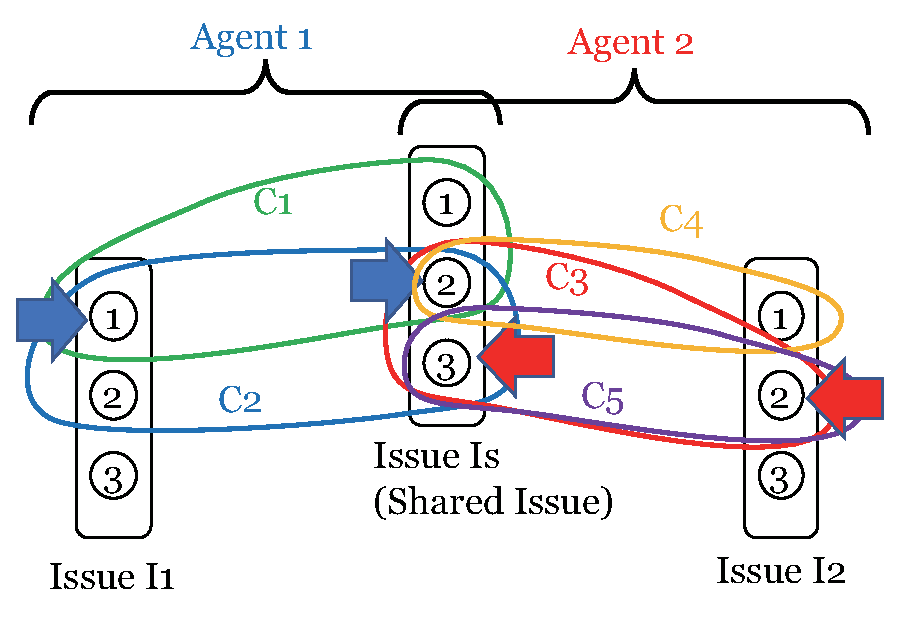
\includegraphics[width=0.45\textwidth]{img/example1.eps}
    \caption{Example of agreement based on constraint relaxation 1: \\Initialization}
    \label{fig:Example1}
\end{figure}
\begin{figure}[h]
    \centering
    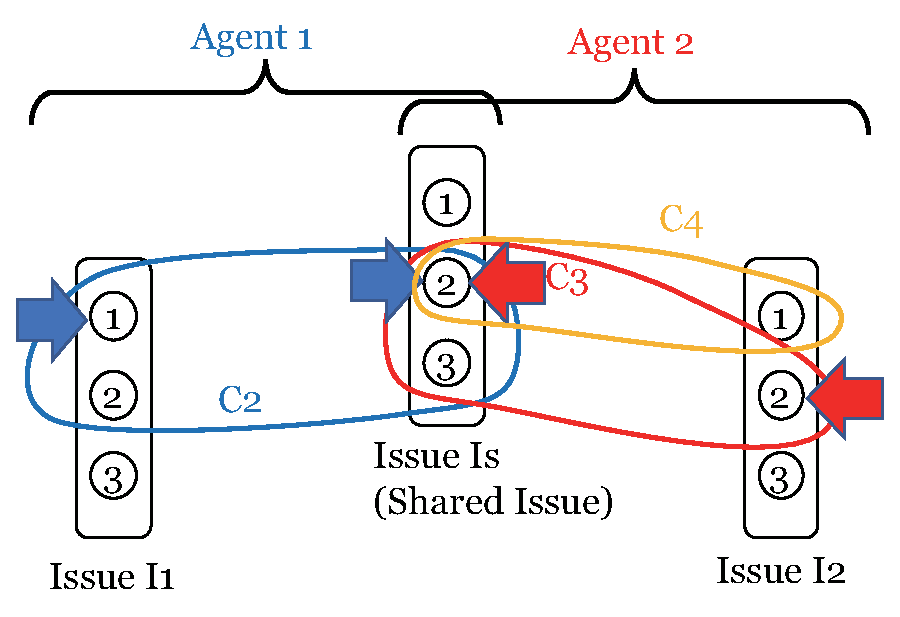
\includegraphics[width=0.45\textwidth]{img/example2.eps}
    \caption{Example of agreement based on constraint relaxation 2: \\Agreement by relaxation}
    \label{fig:Example2}
\end{figure}



 In existing research, no explanation has been provided regarding how the agreement is achieved with these values when making a compromise by ad-hoc threshold adjustment. In this research, satisfiable constraints are reduced. Specifically speaking, we can attain a possible explanation for compromise not by taking the constraint into consideration. therefore, rather evaluating which constraints when taken into consideration, and which constraints when not taken into consideration, would result in an agreement. Essentially, constraints are separated into believed (IN) constraints and non-believed (OUT) constraints. Initially, all constraints are set to IN, while the relaxed constraints are set to OUT.
 
 
%%%%%%%%%%%%%%%%%%%%%%

Fig.\ref{fig:Example1} and Fig.\ref{fig:Example2} show simple examples of the compromise process proposed in this paper. Agent 1 has Issue $I_1$ and Issue $I_s$ as shown in fig.\ref{fig:Example1}. Issue $I_s$ is the shared issue. Agent 2 has Issue $I_2$ and Issue $I_s$. Each issue has issue-values of 1, 2 or 3. Agent 1 has constraints $C_1$ and $C_2$. Since the utility is higher when both issues are satisfied, the initial optimal solution is 1 for $I_1$ and 2 for $I_s$. On the other hand, Agent 2 has constraints $C_3$, $C_4$, and $C_5$. Similarly, the optimal solution is 3 for Issue $I_s$ and 2 for $I_2$. In the case of the Figure 2, agents have the different issue-values for the shared issue $I_s$. Therefore, they have not reached an agreement. Therefore, each agent performs a compromise process by removing one constraint. For example, here, Agent 1 sets constraint $C_1$ to OUT. Agent 2 sets constraint $C_5$ to OUT. Then, Agent 1's $I_s$ issue value stays at 2, whereas Agent 2's $I_s$ issue value also becomes 2. As a result, Agent 1 and Agent 2 reach an agreement. Since it is known which constraints were set to OUT (not believed) in the compromise, it is possible for us to explain which and why constraints were left out. This is different from the existing works in which agents just adjust the threshold of acceptance.



\subsection{A Subsection Sample}

Here, we propose the following four methods. All initial constraints are IN. All initial relaxed constraints are OUT. 


\begin{description}
  \item[Random constraint relaxation\newline(hereinafter, this is called ""random""):] 


One of the constraints in IN is randomly selected and pushed into OUT. 
  \item[Constraint relaxation based on value\\(hereinafter, this is called ""min""):] 


  The lowest value constraint is selected from IN constraints and pushed into OUT. 
  \item[Constraint mitigation based on distance\\(hereinafter, this is called ""distance""):] 


  A constaint which has the longest distance from the shared issue is selected in IN and pushed into OUT. Here, the distance is the number of connected constraints from the shared issue. 
  \item[Constraint relaxation based on value and distance\\(hereinafter, this is called ""min + distance""):] 


  The least value constraint among the most distance constraints from the shared issue is selected from IN and pushed into OUT. 
\end{description}


\section{}
\subsection{}

In this experiment, we compare performaces of the proposed  compromiseing strategies. Our experimental setting is described as follows:\\


There are two agents

 One issue can take max 5 values.
 
 There is a single shared issue. 
 
 Each agent has x issues. 
 
 Each constraint include at least one issue.\\
 
 In other words, each issue is always included in one or more constraints. The number of constraints that include an issue is y. We employ multi-start local search as a search method to find the optimal solution. A graph structure based on constraints and issues are assigned randomly. The above experimental setting implies the situation where there are a lot of issues and these issues are connected with some constraints. But the number of the constraints is small. 



\subsection{}
In this experiment, results are obtained with several settings. Here, two results are shown in fig. 4 and fig5. We compare min, random, distance, and distance +min. In Fig. 4, the number of issues of each agent is x = 1. The number of constraints including an issue is y = 16. In Fig. 5, the number of issues for each agent is x = 2. The number of constraints including an issue is y = 11. In Fig. 6, the number of issues for each agent is x = 1. The number of constraints including each issue is y = 30. In any case, the t-test confirmed that the social welfares for min, distance, and distance-min are significantly higher than the social welfare of random. When the number of issues per agent exceeds 50, we are not able to get a stable experiment result. Namely, it was difficult to obtain a result showing a significant difference in the drawing method. This is the number of points per agent exceeds 50, the number of solutions excezds 
%10^{¥50} 
,and considerable calculation is required to search the optimal solution. Scalabe method would be one of the most important future work. Also, the graph structure currently given to the agent is randomly given. An optimization strategy based on the structure of the graph is also a future work.


\section{}
In this section, we present the differences between our study and the related researches. In the field of automated negotiation researches, the compromise process was first proposed by Klein et al. [18]. His main argument is that it is reasonable for the agent to gradually compromise at the Pareto front in simple negotiations where the issues are independent and the utility space is liner in each issue. But if the issues are interdpendent, it is not simple because utility space is complicated, and which leads the agent to unable to find the Pareto front easily. As one method, Klein et al. proposed the SA based agreement point search protocol (implicitly assuming compromising). In addition, Payemann et al. [19] analyzes various compromise functions. The ANAC Competition [20] has been continued since 2010. It is common for ANAC agents to adopt the method for estimating and presenting proposals that can be statistically accepted from the opponent's offers and accepting the proposal by adjusting the threshold considering the time discount utility. For example, AgentK [21], the winning agent of ANAC 2010, estimates the opponent utility space and the attitude (hostile or compromiser) towards agreement from the opponent's offer history. If the partner seems a compromiser, concession is made, and if the partner is hostile, it will not concede more than a certain threshold. The above is the strategy that pioneered ANAC's basic concession strategy. Fawkes [22] is the winning agent of ANAC 2013. Fawkes estimates optimal concessions using discrete wavelet prediction based on opponent's offer history. The most of the existing works focuses on how to adjust the threshold to accept the opponent offer. The threshold is a kind of the upper limitation utility where the agent can accept the opponent offer. But there is no reason how to realize the threshold value. Thus, they do not explain why the agent compromise. It is a real problem because if your self-driving car compromises, you cannot obtain any explanation on this compromise. Also, as far as the authors know, there is no research that assesses the explanability of compromising in an automated negotiation agent that assumes multi-argument utility functions. There are a series of studies of Katia Sycara [23], [24], [25], [26] which proposed negotiation and compromising processes which can be explainable because they use the case-based reasoning. The point is that they defined compromise and persuasion in the form of logical arguments within the framework of case-based reasoning. A series of studies by Sycara and his/her colleagues is also related to Argumentation theory [27], [28], and it has developed into mathematical argumentation theory. On the other hand, the viewpoint of this research is focusing on how to construct an explainable compromise process based on the utility function that can be handled numerically. he paper [29] proposed DTMS (Distributed Truth Maintenance System) in which they propose a classification of {\it consistency} in multiagent enviroments. It is proposed in the paper [29] proposing DTMS (Distributed Truth Maintenance System) about consistency classification in multi agent environment. They classified the concept of the distributed consistency into Inconsistent, Local-Consistency, Local-and-Shared-Consistency, and Global Consistency. In this study, an agreement means that each agent has its internal consistency while they have a consistent shared issue-value, which is the Local-and-Shared-Consistency. The method of compromising proposed in this paper is one of the methods for obtaining Local-and-Shared-Consistency. However, the constraint graph in this paper repreesnts utility space. On the other hand, DTMS does not express preferences. 


\section{Conclusion}
In this paper, we proposed  an explainable compromise process for automatic negotiation agents. The most of the existing automatic negotiation compromising processes are  ad-hoc adjustments of the threshold to accept the opponent offers. But our proposed method enables to explain it by eliminating constraints one by one. The followings are our contribution:

(1) We have newly proposed an explainable compromise process based on the utility graph that is a graph structure with constraints and issues. 

(2) In automatic multi-issue negotiation, we proposed a new model distinguishing between shared issues and personal issues.

(3) In the compromise process, we proposed a constraint relaxation process based on distance and value and demonstrated its effectiveness.


\bibliographystyle{ieicetr}% bib style
\bibliography{paper}% your bib database



%\begin{thebibliography}{99}% more than 9 --> 99 / less than 10 --> 9



%\bibitem{}
%\end{thebibliography}

%\profile{}{}
%\profile*{}{}% without picture of author's face

\end{document}
